\subsubsection{Dataset Format}

In order to use a multilayer perceptron network, supervised learning must be used in order to let the network learn the function you are trying to represent or approximate. For our project, the network is trained on a set of timeframes corresponding to the wavelet file for an audio track in order to detect beats. A timeframe can be defined as a portion of the audio signal for a music file. Thus, a dataset that mapped different timeframes of an audio file to a beat was required. This required researching into datasets that exposed both the metadata information for a large corpus of  audio files, and the discrete times for when beats occur.\\

With the above requirements, we could define the necessary format of our dataset. Our dataset required pairs of files for an audio track : an uncompressed wavelet file in the ‘.wav’ format and a corresponding ‘.beats’ file containing comma separated times for when beats occurred in a song.\\

\subsubsection{Music Information Retrieval Evaluation Exchange (MIREX)}

Our initial dataset was a small dataset used for a 2012 audio beat tracking competition provided by the Music Information Retrieval Evaluation Exchange (MIREX). MIREX is a contest and conference organized by the graduate school of computer science at the University of Illinois Urbana-Champaign. It provides datasets for contests attempting to identify optimal algorithms for beat detection, tempo change detection and other audio analytics. \\

The dataset used consisted of 100 songs, where each song had a file containing the times when a human audience believe beats occurred. Each audio file was in the uncompressed wavelet format, with 1 audio channel and at a standard 44.1KHz sampling rate of timeframes per second. However each song in this dataset was less than 30 seconds in length, so it did not provide enough timeframes to train any neural network model. \\

\subsubsection{Million Song Dataset}

The Million Song Dataset is a dataset containing audio analysis features for millions of songs. One of the features analyzed and available, is the discrete timing of beats. This dataset is openly available and was produced by the Echo Nost, an audio analytics company. This dataset provided all of the necessary beats information for an incredibly large corpus of songs, 280GB in size. However, unlike the Mirex dataset, it did not provide any media files that would allow us to use as training inputs to our model. Thus, we had to implement our own solution.

\subsubsection{Google Play Music}

In order to build a corpus of media files, we used the GooglePlayMusic API to to download songs. For each song we found in a subset of the MillionSongDataset, we extracted its track title, downloaded the audio file in the MPEG-2 format (mp3), and then converted it to the uncompressed wavelet format. This conversion was performed using the popular FFMPEG utility. 
\begin{center}
	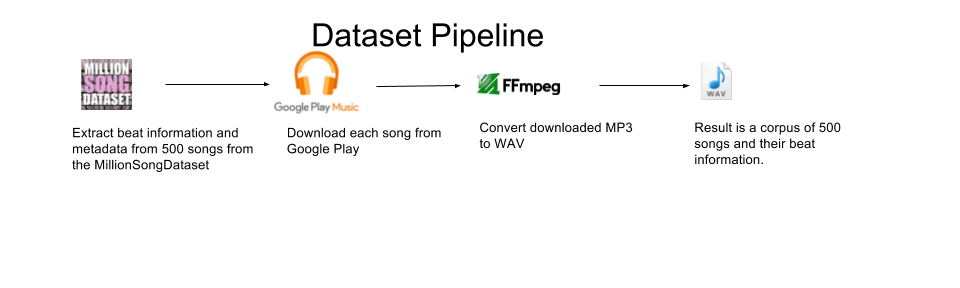
\includegraphics[scale=0.55]{dataset_flow.png}
\end{center}